\newcommand{\nonterminal}[1]{
    \langle \textbf{#1} \rangle
}

\chapter{Zoeken in strings}
\label{ch:zoeken_in_strings}
\begin{itemize}
    \item De gebruikte symbolen:

    \begin{table}[ht]
        \centering
        \begin{tabular}{c l}
            \hline
            Symbool & Betekenis \\
            \hline
            $\Sigma$ & Het gebruikte alfabet \\
            $\Sigma*$ & De verzameling strings van eindige lengte van letters uit $\Sigma$ \\
            d & Aantal karakters in $\Sigma$ \\
            P & Patroon (de tekst die gezocht wordt) \\
            p & Lengte van P \\
            T & De hele tekst waarin gezocht wordt\\
            t & lengte van T \\
            \hline
        \end{tabular}
    \end{table}

    \item We willen een bepaalde string (het patroon P) in een langere string (de tekst T) lokaliseren.
    \item We nemen aan dat we alle plaatsen zoeken waar dat patroon voorkoomt.
    \item We veronderstellen ook dat P en T in het inwendig geheugen opgeslaan zitten.
\end{itemize}


\section{Formele talen}
\begin{itemize}
    \item Een \textbf{formele taal} over een alfabet is een verzameling eindige strings over dat alfabet.
    \item Een formele taal wordt vrij vaag gedefinieerd (maar zien we niet in de cursus).
\end{itemize}

\subsection{Generatieve grammatica's}
\begin{itemize}
    \item Een \textbf{generatieve grammatica} is een methode om een taal te beschrijven.
    \item Er is een startsymbool dat getransformeerd kan worden tot een zin van de taal met behulp van substitutieregels.
    \item Buiten de karakters $\Sigma$ van het alfabet, is er ook nog een verzameling \textbf{niet-terminale symbolen}.
    \item Een niet-terminaal symbool wordt aangeduid als
        $$\nonterminal{\dots}$$
        waarin $\textbf{\dots}$ vervangen wordt door de naam van het niet-terminale symbool. 
    \item De verzameling alle strings uit $\Sigma$ vermengd met de niet-terminale symbolen is $\Xi$, en de daarbijhorende verzameling strings $\Xi*$.
    \item Een belangrijk geval zijn de \textbf{contextvrije grammatica's}.
    \begin{itemize}
        \item Er is op elk moment een string uit $\Xi*$.
        \item Als er geen niet-terminale symbolen meer zijn krijgt men een zin in de taal, anders kan men één niet-terminaal vervangen door een string uit $\Xi*$.
        \item De taal is contextvrij omdat de substitutie onafhankelijk is wat voor en achter de betreffende niet-terminaal staat.
        \item Een voorbeeld van een contextvrije grammatica:

        \begin{align*}
             \nonterminal{S} &::= \nonterminal{AB}\;|\;\nonterminal{CD} \\
             \nonterminal{AB} &::= a\nonterminal{AB}b\;|\;\epsilon \\
             \nonterminal{CD} &::= c\nonterminal{CD}c\;|\;\epsilon
        \end{align*}
        \begin{itemize}
            \item De kleine letters zijn elementen van $\Sigma$ en $\epsilon$ stelt de lege string voor.
            \item Deze grammatica definieert als formele taal de verzameling van alle strings ofwel bestaande uit een rij 'a's gevolgd door een even lange rij 'b's ofwel bestaande uit een rij 'c's gevolgd door een even lange rij 'd's.    
            \item De afleiding van "cccddd":
            $$\nonterminal{S} \rightarrow \nonterminal{CD} \rightarrow c\nonterminal{CD}d \rightarrow cc\nonterminal{CD}dd \rightarrow ccc\nonterminal{CD}ddd \rightarrow cccddd$$
        \end{itemize}
    \end{itemize}
\end{itemize}

\subsection{Reguliere uitdrukkingen}
\begin{itemize}
    \item Een \textbf{reguliere uitdrukking} is ook een methode om een taal te beschrijven.
    \item Een reguliere uitdrukking, of regexp, is een string over het alfabet $\Sigma = \{\sigma_0, \sigma_1, \cdots, \sigma_{d-1}\}$ aangevuld met de symbolen $\varnothing, \epsilon, *, (, )$ en $\bot$, gedefinieerd door
    \begin{align*}
        \nonterminal{Regexp} &::= \nonterminal{basis}\;|\;\nonterminal{samengesteld} \\
        \nonterminal{basis} &::= \sigma_0|\cdots|\sigma_{d-1}|\varnothing|\epsilon \\
        \nonterminal{samengesteld} &::= \nonterminal{plus}|\nonterminal{of}|\nonterminal{ster}\\
        \nonterminal{plus} &::= (\nonterminal{Regexp}\nonterminal{Regexp})\\
        \nonterminal{of} &::= (\nonterminal{Regexp}\bot\nonterminal{Regexp})\\
        \nonterminal{ster} &::= (\nonterminal{Regexp})*
    \end{align*}
    \item Elke regexp $R$ definieert een formele taal, Taal($R$).
    \item Een taal die door een regexp gedefinieerd kan worden heet een reguliere taal.
    \item De definitie van een regexp en reguliere taal is recursief:
    \begin{enumerate}
        \item $\varnothing$ is een regexp, met als taal de lege verzameling.
        \item De lege string $\epsilon$ is een regexp met als taal Taal($\epsilon$) = \{$\epsilon$\}.
        \item  Voor elke $a \in \Sigma$ is 'a' een regexp, met als taal Taal($'a'$) = \{$'a'$\}.
    \end{enumerate}
    \item Regexps kunnen gecombineerd worden via drie operaties:
    \begin{table}[h]
        \centering
        \begin{tabular}{c c c}
            \hline
            Operatie & Regexp & Operatie op taal/talen \\
            \hline
            Concatenatie & (RS) & Taal($R$) $\cdot$ Taal($S$) \\
            Of & (R|S) & Taal($R$) $\cup$ Taal($S$) \\
            Kleenesluiting & (R)* & Taal($R$)* \\
            \hline
        \end{tabular}
    \end{table}
    \item Vaak worden verkorte notaties gebruikt:
    \begin{itemize}
        \item \textbf{Minstens eenmal herhalen}
        $$r+ \leftrightarrow rr*$$
        \item \textbf{Optionele uitdrukking}
        $$r? \leftrightarrow r|\epsilon$$
        
        \item \textbf{Unies van symbolen}
        $$[abc] \leftrightarrow a|b|c$$
        $$[a-z] \leftrightarrow a|b|\dots|z$$

        
    \end{itemize}

    \item Regexps kunnen verbonden worden met graafproblemen.
    \item \textbf{Stelling:} Zij $G$ een gerichte multigraaf met verzameling takken $\Sigma$. Als $a$ en $b$ twee knopen van $G$ zijn dan is de verzameling $P_G(a, b)$ van paden beginnend in $a$ en eindigend in $b$ een reguliere taal over $\Sigma$.
    \item \textbf{Bewijs:}
    \begin{itemize}
        Via inductie op het aantal verbindingen $m$ van $G$.
        \item Als $m = 0$ dan
        $$P_G(a, b) = \begin{cases}
            \{\}, \hbox{ als } a \neq b\\
            \{\epsilon\}, \hbox{ als } a = b 
        \end{cases}$$
        \item Breidt nu de graaf $G$ uit naar $G'$ door één verbinding toe te voegen.
        \begin{itemize}
            \item Een verbinding $v_{xy}$ van knoop $x$ naar knoop $y$, waarbij eventueel $x = y$.
            \item Alle paden van $a$ naar $b$ zijn één van de twee volgende vormen:
            \begin{enumerate}
                \item De paden die $v_{xy}$ niet bevatten. Deze vormen de reguliere taal $P_G(a, b)$.
                \item De paden die $v_{xy}$ wel bevatten. Deze verzameling wordt gegeven door
                $$P_G(a, x) \cdot \{v_{xy}\} \cdot (P_G(y, x) \cdot \{v_{xy}\})* \cdot P_G(y, b)$$

                Deze is bekomen uit reguliere talen en is dus regulier.
            \end{enumerate}
        \end{itemize}
    \end{itemize}
    \item 
\end{itemize}




\section{Variabele tekst}


\subsection{Een eenvoudige methode}
\begin{itemize}
    \item Vanaf positie $j$ in $T$ wordt $P$ vergeleken door de overeenkomstige karakters van beide te vergelijken.
    \item $P[i]$ vergelijken met $T[j + 1]$ voor $0 < i \leq p$.
    \item Stoppen zodra er een verschil is of het einde van $P$ bereikt is.
    \item Dan verder doen voor $j + 1$.
    \item $P[0]$ zal vaak verschillen van $T[j]$, zodat de test op veel beginposities $j$ reeds na één karaktervergelijking stopt.
    \item De gemiddelde uitvoeringstijd is $O(t)$.
    \item In het slechtste geval is dit $O(tp)$.
\end{itemize}


\subsection{Zoeken met de prefixfunctie}
\subsubsection{De prefixfunctie}
\begin{itemize}
    \item Gegeven een string $P$ en index $i$ met $i \leq p$.
    \item Een string $Q$ kan voor $i$ op $P$ gelegd woorden als $i \geq q$ en als $Q$ overeenkomt met de even lange deelstring van $P$ endigend voor $i$.
    \item De index $i$ wijst naar de plaats \textit{voorbij} de deelstring, niet naar de laatste letter van de deelstring.
    \item De prefixfunctie $q()$ van een string $P$ bepaalt voor elke stringpositie $i$, $1 \leq i \leq p$, de lengte van de langste prefix van $P$ met lengte kleiner dan $i$ dat we voor $i$ kunnen leggen.

    \item Volgende eigenschappen gelden:
    \begin{itemize}
        \item $q(i) < i$
        \item $q(1) = 0$
        \item $q(0) = -$ (niet gedefinieerd)
    \end{itemize}
    \item De waarde van $q(i + 1)$ kan bepaald worden als de waarden van de vorige posities gekend zijn.
    $$q(i + 1) = \begin{cases}
        q(i) & \hbox{ als } P[q(i)] = P[i]  \\
        q(q(i)) + 1 & \hbox{ als } P[q(q(i))] = P[i] \\
        q(q(q(i))) + 1 & \hbox{ als } P[q(q(q(i)))] = P[i] \\
        \cdots \\
        0 & \hbox { anders }
    \end{cases}$$

    \begin{itemize}
        \item Stel de string \texttt{ANOANAANOANO}
        \item Dan zijn de waarden van de prefixfunctie als volgt:
        \begin{table}[ht]
            \centering
            \begin{tabular}{l | c c c c c c c c c c c c c}
                     & A & N & O & A & N & A & A & N & O & A  & N  & O  & - \\
                     \hline
                i    & 0 & 1 & 2 & 3 & 4 & 5 & 6 & 7 & 8 & 9 & 10 & 11 & 12  \\
                q(i) & - & 0 & 0 & 0 & 1 & 2 & 1 & 1 & 2 & 3  & 4  & 5 & 3 
            \end{tabular}
        \end{table}
    \end{itemize}
    \item De prefixwaarden worden dus voor stijgende $i$ berekend.
    \item Wat is de \textbf{efficiëntie}?
    \begin{itemize}
        \item Er moeten $p$ prefixwaarden berekend worden.
        \item De recursierelatie wordt ook maar $p-1$ herhaald voor de voltallige bepaling van de prefixfunctie.
        \item De methode is $\Theta(p)$.
    \end{itemize}
\end{itemize}

\subsubsection{Een eenvoudige lineaire methode}
\begin{itemize}
    \item Stel een string samen bestaande uit $P$ gevolgd door $T$, gescheiden door een speciaal karakter dat in niet in beide strings voorkomt.
    \item Bepaal de prefixfunctie van deze nieuwe string, in $\Theta(n + p)$.
    \item Als de prefixwaarde van een positie $i$ gelijk is aan $p$, werd $P$ gevonden, beginnend bij index $i - p$ in $T$.
\end{itemize}


\subsubsection{Het Knuth-Morris-Prattalgoritme}
\begin{itemize}
    \item Ook een lineaire methode, maar is efficiënter.
    \item Stel dat $P$ op een bepaalde beginpositie vergeleken wordt met $T$, en dat er geen overeenkomst meer is tussen $P[i]$ en $T[j]$.
    \begin{itemize}
        \item Als $i = 0$, dan wordt $P$ één positie naar rechts geschoven en begint het vergelijken met $T$ weer bij $P[0]$.
        \item Als $i > 0$, dan is er een prefix van $P$ met lengte $i$ gevonden, dat we voor $j$ op $T$ kunne leggen.
        \begin{itemize}
            \item Verschuif $P$ met een stap $s$ kleiner dan $i$.
            \item Er is nu een overlapping tussen het begin van $P$ en het prefix van $P$ dat we in $T$ gevonden hebben.
            \item De overlapping heeft lengte $i - s$.
            \item De overlappende delen moeten wel overeenkomen.
            \item De kleinste waarde van $s$ waarbij dit mogelijk is, is $s = i - q(i)$.
        \end{itemize}
    \end{itemize}
\end{itemize}


\subsection{Onzekere algoritmen}
\begin{itemize}
    \item Algoritmen die een zekere waarschijnlijkheid hebben om een geheel foutief resultaat te geven.
    \item Zulke algoritmen worden ook \textbf{Monte Carloalgoritmen} genoemd.
    \item Er zijn redenen waarom zulke algoritmen toch nuttig kunnen zijn;
    \begin{enumerate}
        \item Zulke algoritmen zijn vaak sneller.
        \begin{itemize}
            \item Een voorbeeld is een \textbf{Bloomfilter}.
            \item We willen een verzameling van objecten in gehashte vorm bijhouden.
            \item Een Bloomfilter houdt de logische bitsgewijze OF bij van de hashwaarden van alle elementen.
            \item Om te weten of een object in de verzameling zit wordt deze eerst gehasht. Daarna wordt de logische EN operatie gebruikt op de bloomfilter met deze waarde.
            \item Als het resultaat verschilt van de hashwaarde dan zit het object er zeker niet in.
            \item Anders weten we het niet.
        \end{itemize}
        \item Men tracht de kans dat er een fout voorkomt zo klein mogelijk te maken.
    \end{enumerate}
\end{itemize}


\subsection{Het Karp-Rabinalgoritme}
\begin{itemize}
    \item Herleidt het vergelijken van strings tot het vergelijken van getallen.
    \item Aan elke mogelijke string die even lang is als $P$ wordt een uniek getal toegekend.
    \item In plaats van $P$ en de even lange deeltekst op een bepaalde positie te vergelijken, worden de overeenkomstige getallen vergeleken.
    \item Gelijke strings betekent gelijke getallen en omgekeerd is dit ook waar.
    \item Er zijn $d^p$ verschillende strings met lengte $p$, zodat de getallen groot kunnen worden.
    \item Daarom worden de getallen beperkt tot deze die in één processorwoord (met lengte $w$ bits) voorgesteld kunnen worden.
    \item Meerdere strings zullen met hetzelfde getal moeten overeenkomen ($\equiv$ hashing).
    \item Gelijke strings betekent nog altijd gelijke getallen, maar een gelijk getal betekent niet meer dezelfde string.
    \item Af en toe vergissen is dus mogelijk.
    \item Hoe worden de getallen gedefinieerd?
    \begin{itemize}
        \item Ze moeten in $O(1)$ berekend kunnen worden voor elk van de $O(t)$ deelstrings in de tekst.
        \item Een hashwaarde voor een string met lengte $p$ in $O(1)$ berekenen is niet realistisch.
        \item Daarom wordt de hashwaarde voor de deelstring op positie $j + 1$ berekend op basis van de deelstring op basis $j$.
        \item De eerste hashwaarde berekenen ($j = 0$) mag dan langer duren.
    \end{itemize}
    

    \item De voorstelling van $P$:
    \begin{itemize}
        \item We beschouwen een string als een getal in een $d-$tallig talstelsel omdat elk stringelement $d$ waarden kan aannemen zodat elk stringelement wordt voorgesteld door een cijfer tussen 0 en $d - 1$.
        
        $$H(P) = \sum_{i=0}^{p-1} P[i]d^{p-i-1} = P[0]d^{p-1} + P[1]d^{p-2} + \dots + P[p-2]d + P[p-1]$$

        \item Om de beperkte waarde te bekomen, wordt de rest bij deling door een getal $r$ genomen. Dit wordt de \textbf{fingerprint} genoemd.
        $$H_r(P) = H(P)\;\mathrm{mod}\;r$$
    
        \item Dit is geen efficiënte operatie omdat de individuele getallen van de som in $H(p)$ groot kunnen worden, maar gelukkig
        $$(a + b) \;\mathrm{mod}\;r = (a\;\mathrm{mod}\;r + b\;\mathrm{mod}\;r)\;\mathrm{mod}\;r$$
    
        Dit geldt ook voor verschil en het product.
    
        \item Omdat elk tussenresultaat nu binnen een processorwoord past, is $H_r(P)$ berekenen slechts $\Theta(P)$.
    \end{itemize}
    \item De voorstelling van $T$:
    \begin{itemize}
        \item De waarde $T_0$ bij beginpositie $j = 0$ wordt op dezelfde manier berekend als $P$.
        $$H(T_0) = \sum_{i=0}^{p-1} T[i]d^{p-i-1} = T[0]d^{p-1} + T[1]d^{p-2} + \dots + T[p-2]d + T[p-1]$$

        \item Er is nu een eenvoudig verband tussen het getal voor de deelstring $T_{j + 1}$ bij beginpositie $j + 1$ en dat voor $T_{j}$ bij beginpositie $j$:

        $$H(T_{j + 1}) = (H(T_j) - T[j]d^{p-1})d + T[j + p]$$

        (term met de hoogste macht aftrekken en die met de kleinste opstellen)

        \begin{itemize}
            \item Stel een string T = \texttt{ABCDE}, $d = 5$ en $p$ = 3 (wat $P$ is maakt niet uit voor dit voorbeeld). De waarden van de stringelementen zijn $A = 1, B = 2, C = 3, D = 4, E = 5$.
            \item De opeenvolgende waarden $T_j$ zijn dan:
            \begin{itemize}
                \item \begin{align*}
                    H(T_0) &= \sum_{i=0}^{2} T[i]5^{2-i}\\
                    & = A\cdot 5^2 + B\cdot 5^1 + C\\
                    & = 1\cdot 5^2 + 2\cdot 5^1 + 3\\
                    &= 25 + 10 + 3 = 38
                \end{align*}
                \item \begin{align*}
                    H(T_1) &= (H(T_0) - T[0]5^{2})\cdot 5 + T[3]\\
                           &= (A\cdot 5^2 + B\cdot 5 + C - A\cdot 5^2)\cdot 5 + D \\
                           &= B\cdot 5^2 + C \cdot 5 + D  \\
                           &= 2\cdot 5^2 + 3 \cdot 5 + 4  \\
                           &=  50 + 15 + 4 = 69
                \end{align*}
                \item \begin{align*}
                    H(T_2) &= (H(T_1) - T[1]5^{2})\cdot 5 + T[4]\\
                           &= (B\cdot 5^2 + C\cdot 5 + D - B\cdot 5^2)\cdot 5 + E \\
                           &= C\cdot 5^2 + D \cdot 5 + E  \\
                           &= 3\cdot 5^2 + 4 \cdot 5 + 5  \\
                           &=  75 + 20 + 5 = 100
                \end{align*}
            \end{itemize}
            
            
        \end{itemize}

        \item De fingerprint is dan
        $$H_r(T_{j + 1}) = ((H(T_j) - T[j]d^{p-1})d + T[j + p])\;\mathrm{mod}$$

        \item Het berekenen van $H_r(P)$, $H(T_0)$ en $d^{p-1}\;\mathrm{mod}\;r$ vereist $\Theta(p)$ operaties.
        \item Het berekenen van alle andere fingerprints $H_r(T_j) (0 < j \leq t - p)$ vergt $\Theta(t)$ operaties.
        \item Dit is $\Theta(t + p)$.
        \item Maar, de strings moeten nog vergeleken worden als de fingerprints hetzelfde zijn.
        \item In het slechtste geval zijn de fingerprints op elke positie gelijk, zodat de totale performantie $\textbf{O(tp)}$ is.
        \item Er zijn nu nog twee mogelijkheden om $r$ te bepalen:
        \begin{enumerate}
            \item \textbf{Vaste $r$}
            \begin{itemize}
                \item Kies $r$ als een zo groot mogelijk priemgetal zodat $rd \leq 2^w$.
                \item Priemgetallen zorgt ervoor dat gelijkaardige deelstrings dezelfde fingerprinters zouden opleveren.
                \item Een groot priemgetal zorgt voor een groot aantal mogelijke fingerprints.
                \item Er is nu wel een nieuw verband tussen $H_r(T_{j + 1})$ en $H_r(T_j)$:
                $$H_r(T_{j + 1}) = \bigg(\big((H_r(T_j) + r(d - 1) - T[j](d^{p-1}\;\mathrm{mod}\;r)) \;\mathrm{mod}\;r\big)d + T[j + 1] \bigg)\;\mathrm{mod}\;r$$
                
                (De term $r(d - 1)$ wordt toegevoegd om een negatief tussenresultaat te vermijden.)
            \end{itemize}


            \item \textbf{Random $r$}
            \begin{itemize}
                \item Soms is een vaste $r$ nadelig: er kan bijvoorbeeld een slechte waarde gekozen worden.
                \item De veiligste implementatie gebruikt een willekeurige priem $r$ uit een bepaald bereik.
                \item Een groter bereik reduceert de kans op fouten.
                \item Het aantal priemgetallen kleiner of gelijk aan $k$ is $\frac{k}{\ln k}$.
                \item Door $k$ groot te kiezen zal slechts een klein deel van die priemgetallen een fout veroorzaken.
                \item De kans dat $r$ één van die priemen is wordt klein.
                \item Voor $k = t^2$ is de kans op één enkele foute $O(1/t)$.
                \item Om fouten helemaal te vermijden zijn er twee mogelijkheden:
                \begin{itemize}
                    \item Overgaan naar een andere methode als de fout gesignaleerd wordt.
                    \item Herbeginnen met een nieuwe random priem $r$.
                \end{itemize}
            \end{itemize}
        \end{enumerate}

    \end{itemize}

\end{itemize}


\subsection{Zoeken met automaten}
\begin{itemize}
    \item Automaten beschrijven algemene informatieverwerkende eenheden met een eindig geheugen.
    \item Het geheugen wordt voorgesteld door \textbf{staten}.
    \begin{itemize}
        \item Er zijn evenveel staten als er mogelijkheden zijn.
        \item Een geheugenmodule van 32 kilobyte heeft $256^{32000}$ mogelijke staten.
    \end{itemize}
    \item Een automaat modelleert ook de tijd als een 

    \item \textbf{Deterministische automaten.}
    \begin{figure}[ht]
        \centering
        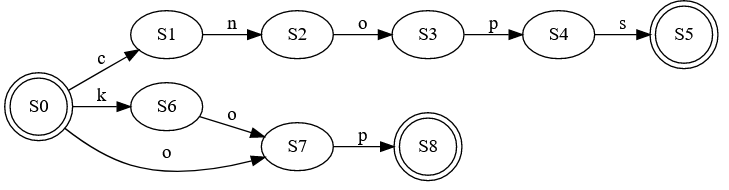
\includegraphics[width=0.7\textwidth]{deterministic_automata}
        \caption{Een deterministische automaat die de woorden \texttt{CNOPS}, \texttt{KOP} en \texttt{OP} herkent. $S_0$ is de startstaat, $S_5$ en $S_8$ zijn eindstaten.}
        \label{fig:deterministic_automata}
    \end{figure}
    \begin{itemize}
        \item Een deterministische automaat (DA) bestaat uit:
        \begin{itemize}
            \item Een (eindige) verzameling invoersymbolen $\Sigma$.
            \item Een (eindige) verzameling toestanden $S$.
            \item Een begintoestand $s_0 \in S$.
            \item Een verzameling eindtoestanden $F \subset S$.
            \item Een overgangsfunctie $p(t, a)$ die een nieuwe toestand geeft wanneer de automaat in staat $t$ symbool $a$ ontvangt.
        \end{itemize}
        \item Een DA wordt voorgesteld door een gerichte geëtiketteerde multigraaf $G$, de \textbf{overgangsgraaf}.
        \begin{itemize}
            \item De knopen zijn de verschillende staten.
            \item De verbindingen zijn de overgangen met als etiket het overeenkomstig invoersymbool.
        \end{itemize}
        \item Een DA start altijd in zijn begintoestand, en maakt de gepaste toestandsovergangen bij elk ingevoerd symbool.
        \item Als een DA zich in een eindtoestand bevindt, dan wordt de string \textbf{herkend} door de DA. De verzameling strings die herkend wordt door een DA is de taal van die automaat.
    \end{itemize}

    \item \textbf{Niet-deterministische automaten.}
    \begin{itemize}
        \item Heeft geen staten, maar wel \textbf{statenbits}.
        \item De 'staat' van een NA wordt aangeduid door de verzameling statenbits die aan staan.
        \item De beginstaat wordt aangeduidt met een speciale statenbit, de beginbit, die aanstaat in het begin terwijl alle andere uit staan.
        \item De eindstaten worden aangeduid door de eindbits.
        \item De overgang van een staat naar de volgende werkt bit per bit.
        \item Een statenbit die aan staat reageert op een invoersymbool door een signaal naar nul of meer statenbits te sturen.
        \item Een statenbit die één of meer signalen binnekrijgt zet zichzelf aan, anders uit.
        \item Als $i$ een statenbit is en $a$ een letter uit het alfabet, dan is $s(i, a)$ de verzameling statenbits die rechtstreeks een signaal van $i$ krijgen als de inkomenden letter $a$ is.
        \item Er zijn ook $\epsilon-$overgangen. Een $\epsilon-$overgang van statenbit $i$ naar statenbit $j$ zorgt ervoor dat $i$ direct een signaal uitstuurt naar $j$, zonder vertraging.
    \end{itemize}

    \begin{figure}[ht]
        \centering
        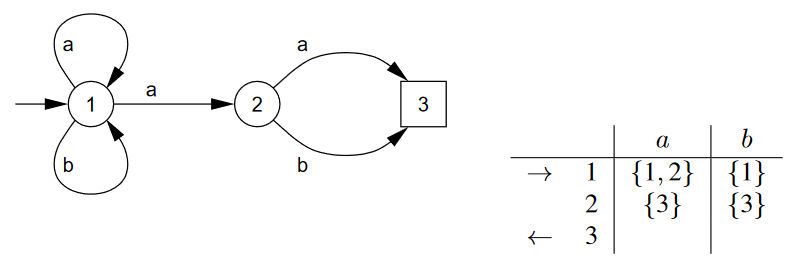
\includegraphics[width=\textwidth]{nondeterministic_automata}
        \caption{Een niet-deterministische automaat en bijhorende statentabel voor de reguliere expressie $(a|b)*a(a|b)$.}
        \label{fig:nondeterministic_automata}
    \end{figure}
\end{itemize}

\subsubsection{De deelverzamelingconstructie}
\begin{itemize}
    \item Een NA is een alternatieve voorstelling van een DA, maar laat geen efficiënte implementatie toe:
    \begin{itemize}
        \item Bij elke binnenkomende letter moeten alle statenbits die aanstaan overlopen worden, en de daarbijhorende bits die een signaal krijgen aanduiden.
        \item Bij een DA moet voor elke binnenkomende letter enkel de nieuwe staat opgezocht worden in de tabel.
    \end{itemize}
    \item Een NA is wel eenvoudiger om op te stellen. Een reguliere uitdrukking kan eenvoudig omgezet worden tot een NA.
    \item \textbf{Een NA omzetten naar een DA} wordt de \textbf{deelverzamelingconstructie} genoemd.
    \begin{figure}[ht]
        \centering
        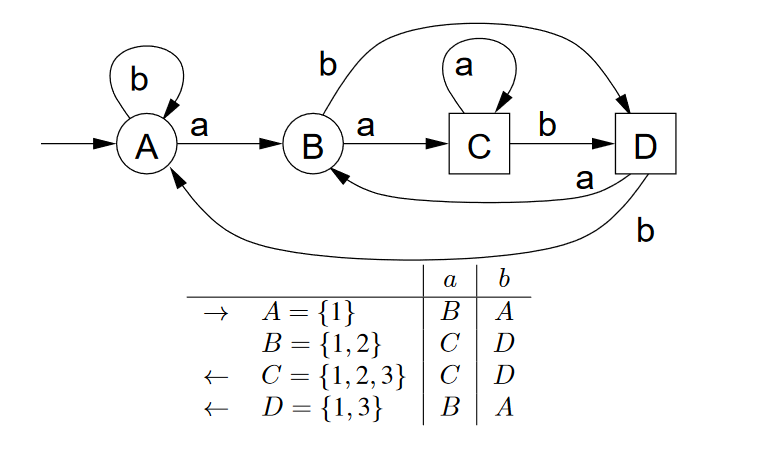
\includegraphics[width=0.7\textwidth]{deterministic_automata_2.PNG}
        \caption{De deterministische automaat geconstrueerd uit die van figuur \ref{fig:nondeterministic_automata}.}
        \label{fig:deterministic_automata_2.PNG}
    \end{figure}
    \begin{itemize}
        \item Als een NA $k$ statenbits heeft, zijn er $2^k$ mogelijke deelverzamelingen.
        \item Die allemaal nagaan is niet efficiënt aangezien de meeste deelverzamelingen al niet bereikbaar zijn vanuit de begintoestand. Op figuur \ref{fig:nondeterministic_automata} is te zien dat enkel de deelverzamelingen \{1\}, \{1, 2\} en \{3\} (3 van de 8 deelverzamelingen) op elk moment beschikbaar kunnen zijn. 
        \item Er is dus een implicite multigraaf met $2^k$ knopen die doorlopen kan worden met breedte-eerst of diepte-eerst zoeken.
        \item Knopen die niet bereikbaar zijn zijn overbodig voor de DA.
        \item Buren in deze impliciete multigraaf kunnen niet opgezocht worden in een burenlijst. Er zijn hulpoperaties nodig:
        \begin{itemize}
            \item De \textbf{$\epsilon-$sluiting(T)} geeft de deelverzameling van statenbits bereikbaar via $\epsilon-$overgangen vanuit een verzameling statenbits $T$ (gewoon via diepte eerst zoeken zoals pseudocode 11.1 in cursus).
            \item De overgangsfunctie $p(t, a)$ kan uitgebreidt worden voor een verzameling van statenbits tot $p(T, a)$: de deelverzameling van alle statenbits rechtstreeks bereikbaar vanuit een toestand $t$ uit $T$ voor het invoersymbool $a$.
        \end{itemize}
        \item Voor een DA hebben we verzameling van toestanden $D$ en overgangstabel $M$ nodig.
        \item De begintoestand van de DA is $\epsilon-$sluiting($b_0$).
        \item dunno man
    \end{itemize}
    
\end{itemize}

\subsection{De Shift-AND-methode}
\begin{itemize}
    \item Bitgeoriënteerde methode, die efficiënt werkt voor \textbf{kleine patronen}.
    \item Voor elke positie $j$ in de tekst $T$ bijhouden welke prefixen van het patroon $P$ overeenkomen met de tekst, eindigend op positie $j$.
    \item Maakt gebruik van een tabel $R$ met $p$ logische waarden. Het $i-$de element komt overeen met prefix van lengte $i$.
    \begin{itemize}
        \item $R_j$ stelt de waarde van tabel $R$ na verwerking van $T[j]$.
        \item $R_j[i - 1]$ is waar als de eerste $i$ karakters van $P$ overeenkomen met de $i$ testkarakters eindigend in $j$.
        \item De tabel $R_{j+1}$ kan afgeleidt worden uit $R_j$, aangezien sommige prefixen verlengd kunnen worden:
        \begin{align*}
            R_{j + 1}[0] & = \begin{cases}
                1, \hbox{ als } P[0] = T[j + 1] \\
                0, \hbox{ als } P[0] \neq T[j + 1] \\
            \end{cases}\\
            R_{j + 1}[i] & = \begin{cases}
                1, \hbox{ als } R_{j - 1} = 1 \hbox{ en } P[i] = T[j + 1] \\
                0, \hbox{ anders }
            \end{cases} 
            \qquad \hbox{ voor } 1 \leq i \leq p
        \end{align*}
    \end{itemize}
    \item Bij de berekening van $R_{j + 1}$ moeten we weten of $T[j + 1]$ gelijk is aan $P[i]$, voor elke mogelijke waarde van $i$.
    \item Er wordt een tweedimensionaletabel $S$ opgesteld met $d$ (lengte van alfabet) bitpatronen. Een bit $i$ van woord $S[s]$ is waar als het karakter $s$ op plaats $i$ in $P$ voorkomt.

    \item Om alle bits $R_{j + 1}$ gelijktijdig te berekenen wordt de schuifoperatie naar rechts gebruikt (bit $i$ wordt bit $i + 1$, en er wordt vooraan een éénbit ingeschoven), gevolgd door een bit-per-bit EN-operatie met $S[T[j + 1]]$
    
    $$R_{j + 1} = \hbox{Schuif}(R_j) \hbox{ EN } S[T[j + 1]]$$

    \item \textbf{Voorbeeld:}
    \begin{itemize}
        \item Stel $\Sigma = \{A, C, G, T\}$ en $d = 4$.
        \item Stel $P = $ \texttt{GCAGAGAG}.
        \item Stel $T = $ \texttt{GCATCGCAGAGAGTATACAGTACG}.
        \item De tabel $S$ kan uit $P$ berekent worden:
        \begin{table}[ht]
            \centering
            \begin{tabular}{|c | c c c c |}
                \hline
                & $S[A]$ & $ S[C]$ & $ S[G]$ & $S[T]$ \\
                \hline
                G & 0 & 0 & 1 & 0 \\
                C & 0 & 1 & 0 & 0 \\
                A & 1 & 0 & 0 & 0 \\
                G & 0 & 0 & 1 & 0 \\
                A & 1 & 0 & 0 & 0 \\
                G & 0 & 0 & 1 & 0 \\
                A & 1 & 0 & 0 & 0 \\
                G & 0 & 0 & 1 & 0 \\
                \hline
            \end{tabular}
        \end{table}
        \item De tabellen $R_j$ worden dan:

        \begin{table}[ht]
            \centering
            \scalebox{0.6}{
            
            \begin{tabular}{|c c | c c c c c c c c c c c c c c c c c c c c c c c c |}
                \hline
                & & $R_0$&$R_1$&$R_2$&$R_3$&$R_4$&$R_5$&$R_6$&$R_7$&$R_8$&$R_9$&$R_{10}$&$R_{11}$&$R_{12}$&$R_{13}$&$R_{14}$&$R_{15}$&$R_{16}$&$R_{17}$&$R_{18}$&$R_{19}$&$R_{20}$&$R_{21}$&$R_{22}$&$R_{23}$\\
                & & G&C&A&T&C&G&C&A&G&A&G&A&G&T&A&T&A&C&A&G&T&A&C&G\\
                \hline
                $R[0]$ & G & \textbf{1} & 0&0&0&0&\textbf{1}&0&0&\textbf{1}&0&\textbf{1}&0&\textbf{1}&0&0&0&0&0&0&\textbf{1}&0&0&0&\textbf{1}  \\
                $R[1]$ & C & 0 & \textbf{1}&0&0&0&0&\textbf{1}&0&0&0&0&0&0&0&0&0&0&0&0&0&0&0&0&0  \\
                $R[2]$ & A & 0 & 0&\textbf{1}&0&0&0&0&\textbf{1}&0&0&0&0&0&0&0&0&0&0&0&0&0&0&0&0  \\
                $R[3]$ & G & 0 & 0&0&0&0&0&0&0&\textbf{1}&0&0&0&0&0&0&0&0&0&0&0&0&0&0&0  \\
                $R[4]$ & A & 0 & 0&0&0&0&0&0&0&0&\textbf{1}&0&0&0&0&0&0&0&0&0&0&0&0&0&0  \\
                $R[5]$ & G & 0 & 0&0&0&0&0&0&0&0&0&\textbf{1}&0&0&0&0&0&0&0&0&0&0&0&0&0  \\
                $R[6]$ & A & 0 & 0&0&0&0&0&0&0&0&0&0&\textbf{1}&0&0&0&0&0&0&0&0&0&0&0&0  \\
                $R[7]$ & G & 0 & 0&0&0&0&0&0&0&0&0&0&0&\textbf{1}&0&0&0&0&0&0&0&0&0&0&0  \\
                
                \hline
            \end{tabular}
            }
        \end{table}
        \begin{itemize}
            \item Start vanuit $R_0 = \begin{bmatrix}1&0&0&0&0&0&0&0\end{bmatrix}$ (want $R_0[0] = P[0]$).
            \begin{align*}
                R_{1} & = \hbox{Schuif}(R_0) \hbox{ EN } S[T[1]] \\
            & = \begin{bmatrix}1& 1& 0& 0& 0& 0& 0& 0\end{bmatrix} \hbox{ EN } \begin{bmatrix}0&1&0&0&0&0&0&0\end{bmatrix} \\
                      & = \begin{bmatrix}0&1&0&0&0&0&0&0\end{bmatrix} \\
                R_{2} & = \hbox{Schuif}(R_1) \hbox{ EN } S[T[2]] \\
                      & = \begin{bmatrix}1&0&1&0&0&0&0&0\end{bmatrix} \hbox{ EN } \begin{bmatrix}0&0&1&0&1&0&1&0\end{bmatrix} \\
                      & = \begin{bmatrix}0&0&1&0&0&0&0&0\end{bmatrix}\\
                R_{3} & = \hbox{Schuif}(R_2) \hbox{ EN } S[T[3]] \\
                      & = \begin{bmatrix}1&0&0&1&0&0&0&0\end{bmatrix} \hbox{ EN } \begin{bmatrix}0&0&0&0&0&0&0&0\end{bmatrix} \\
                      & = \begin{bmatrix}0&0&0&0&0&0&0&0\end{bmatrix} \\
                R_{4} & = \hbox{Schuif}(R_3) \hbox{ EN } S[T[4]] \\
                      & = \begin{bmatrix}1&0&0&0&0&0&0&0\end{bmatrix} \hbox{ EN } \begin{bmatrix}0&1&0&0&0&0&0&0\end{bmatrix} \\
                      & = \begin{bmatrix}0&0&0&0&0&0&0&0\end{bmatrix} \\
                R_{5} & = \hbox{Schuif}(R_4) \hbox{ EN } S[T[5]] \\
                      & = \begin{bmatrix}1&0&0&0&0&0&0&0\end{bmatrix} \hbox{ EN } \begin{bmatrix}1&0&0&0&0&0&0&0\end{bmatrix} \\
                      & = \begin{bmatrix}1&0&0&0&0&0&0&0\end{bmatrix} \\
                      \cdots \\
                R_{8} & = \hbox{Schuif}(R_7) \hbox{ EN } S[T[8]] \\
                      & = \begin{bmatrix}1&0&0&1&0&0&0&0\end{bmatrix} \hbox{ EN } \begin{bmatrix}1&0&0&1&0&1&0&1\end{bmatrix} \\
                      & = \begin{bmatrix}1&0&0&1&0&0&0&0\end{bmatrix}\\
                      \cdots \\
                R_{12} & = \hbox{Schuif}(R_{11}) \hbox{ EN } S[T[12]] \\
                      & = \begin{bmatrix}1&0&0&0&0&0&0&1\end{bmatrix} \hbox{ EN } \begin{bmatrix}1&0&0&1&0&1&0&1\end{bmatrix} \\
                      & = \begin{bmatrix}1&0&0&1&0&0&0&\textbf{1}\end{bmatrix}
            \end{align*}

        \end{itemize}

        \item Bij $R_{12}$ is $R_{12}[7] = 1$, zodat $P$ gevonden is en begint in $T$ op positie $T[12 - 7] = T[5]$.
    \end{itemize}
    \item De totale performantie is $\textbf{\Theta(t + p)}$
\end{itemize}


\section{De Shift-AND methode: benaderende overeenkomst}
\begin{itemize}
    \item De Shift-AND methode kan aangepast worden om fouten in het gevonden patroon toe te laten.
    \item Veronderstel dat er één karakter op een willekeurige plaats in $P$ mag vervangen worden.
    \begin{itemize}
        \item We zoeken dus alle deelstrings in $T$ niet langer dan $m + 1$ die $P$ als deelsequentie bevatten.
        \item Er is een nieuwe tabel $R_j^1$ die alle prefixen aanduidt in de tekst eindigend bij positie $j$, met hoogstens één vervanging.
        \item $R_j^1[i]$ is waar als de eerste $i$ karakters van $P$ overeenkomen met de $i$ van de $i + 1$ karakters die in de tekst eindigen bij positie $j$.
    \end{itemize}
\end{itemize}